\clearpage{\pagestyle{empty}\cleardoublepage}

\chapter{Event reconstruction}\label{chap:objects}

After having described the ATLAS detector in Chapter~\ref{chap:atlas} 
and the procedure for Monte Carlo simulation of events in Chapter~\ref{chap:mc},
we understand that what we deal with when we talk about ``data'' 
is raw digital signals from the detector,
either the real one or the simulated one.

In the following Chapter we will explain how, starting from these outputs,
objects are reconstructed to be used in physics analyses~\cite{Aad:2009wy}. 
This process is what is called ``offline event reconstruction'' since
it is not done in real time, due to the time required by the algorithms
to perform their tasks.

In general we could describe the full procedure as subdivided into
three main steps: a pre-reconstruction stage where the electronic signals are
translated into measurements; a pattern-recognition step where the measurements
are assembled into the building blocks of particles, e.g. tracks and energy clusters;
a particle identification final leg where the full detector information elaborated 
is combined to match a candidate physics object 
(electrons, muons, jets and the missing transverse energy \met).

The expected signatures for the various particles in terms of interaction
with the detector system are schematically shown in Figure~\ref{fig:decaychart}.

\begin{figure}[tb]\begin{center}
        \subfigure{
  	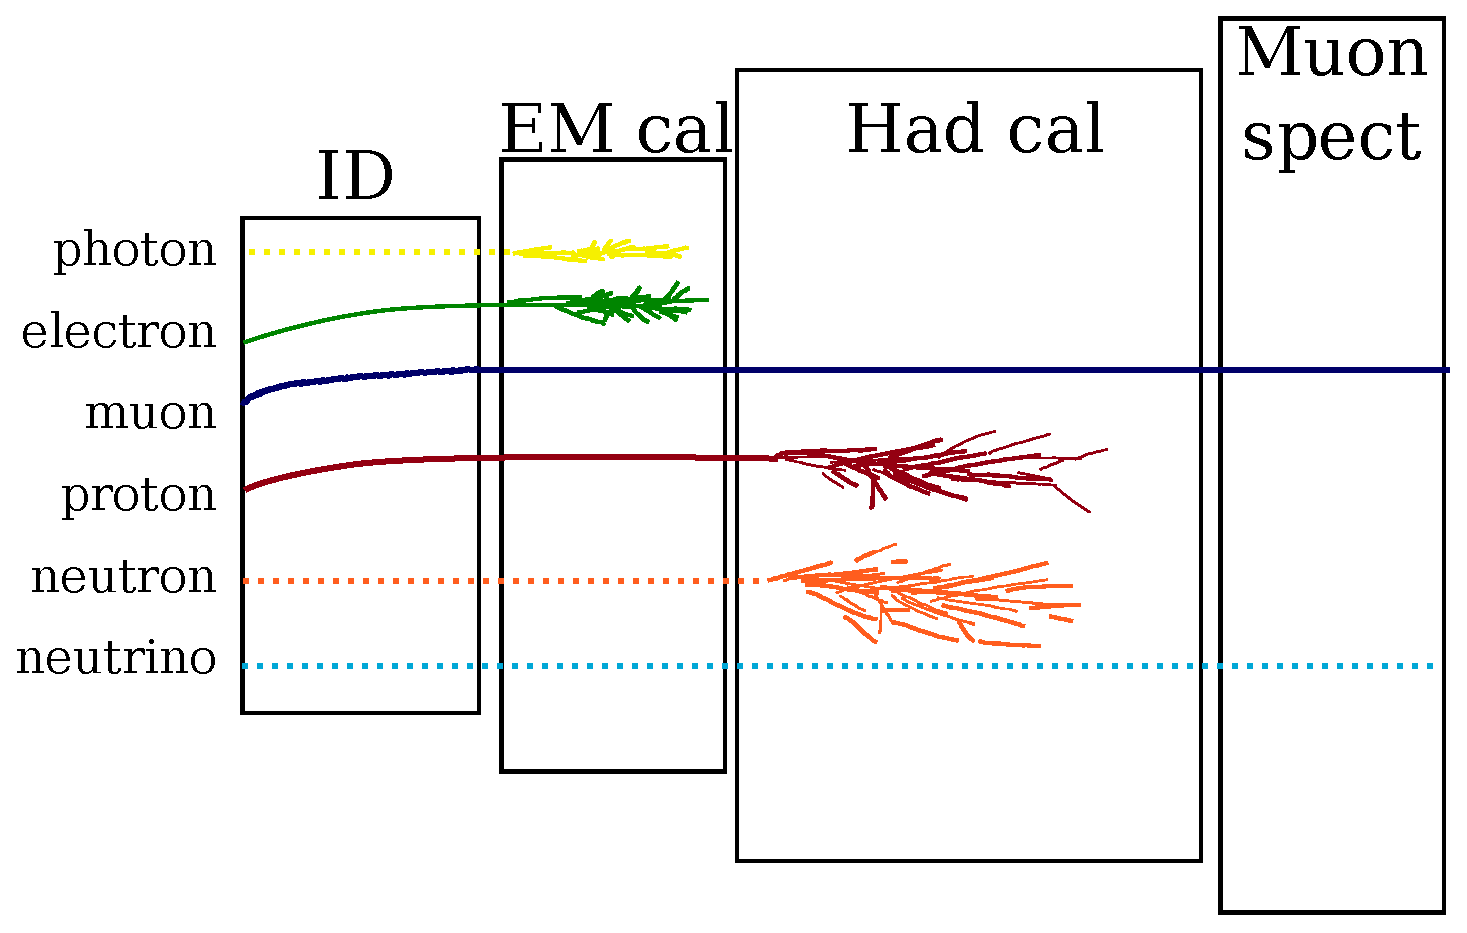
\includegraphics[width=0.7\textwidth]{objectsreconstruction/figures/particles}}
	\caption{Drawing illustrating how particles are detected in the ATLAS sub-systems.
	\label{fig:decaychart}}
\end{center}\end{figure}

%In addition, some details from
%selections specific for the analyses presented in this dissertation will be given.

\section{ID Tracks}\label{sec:tracks}

Particle trajectories (``tracks'') are used both to reconstruct the particle itself, giving the 
momentum measurement, and to identify the interaction vertices.
The parameters describing a track are: $q/p$, the charge divided by the momentum; $\theta$, or more used $\eta$, the angle
with respect to the Z axis in the $R$Z plane measured from the 
perigee\footnote{The perigee is the point of the track closest to the origin.}; $\phi_0$, the angle 
with respect to the X axis in the XY plane measured from the perigee; $d_0$, the impact parameter, 
or perigee with respect to the Z axis in the XY plane; $z_0$, Z component of the perigee.
These parameters are shown in the double-view drawing of Figure~\ref{fig:trackpar}.

\begin{figure}[tb]\begin{center}
	\subfigure{
  	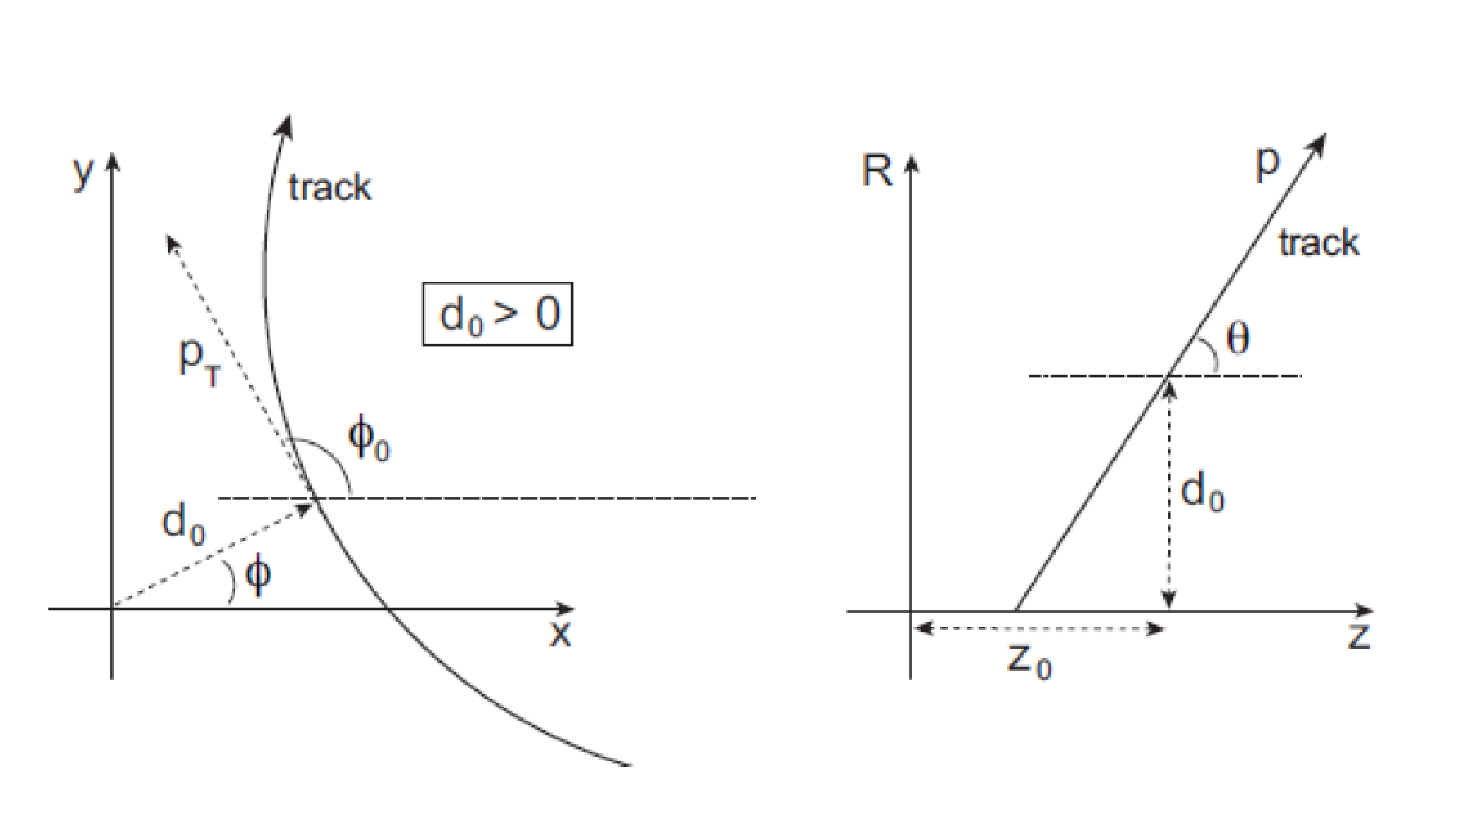
\includegraphics[width=0.7\textwidth]{objectsreconstruction/figures/tracks}}
	\caption[bla]{Schematic drawings of the parameters used for track reconstruction in the XY and $R$Z planes (left and right respectively)
          where the origin is the beam spot, i.e. where the protons collide and interact.
\label{fig:trackpar}}
\end{center}\end{figure}

In order to reconstruct the track, the first step is to retrieve the information from
the ID hits, which are converted into three-dimensional space points. Then, 
the {\it inside-out} algorithm~\cite{Cornelissen:1020106} is used, starting from a
seed of three aligned hits in the pixel detector or in the SCT.
From there, a path is formed along the seed directional information adding
space points one by one. This is done by using a Kalman filter algorithm~\cite{Frühwirth1987444}
which checks progressively the compatibility between the track (also progressively updated)
and the new point. The five track parameters described before are also computed at this step.
%As basic requirements, the candidate track must be formed by at least seven points
%measured in the silicon detectors, $d_0$ must be lower than 10~mm and the 
%transverse momentum must be higher than 150~\mev.  
A cleaning procedure then 
rejects incomplete tracks or tracks sharing hits with others, or composed by
false space points. The candidate tracks are extended
into the TRT and re-fitted taking into account the effects from the interaction
of the charged particle with the detector material. 
%If at least ten TRT hits
%within 10~mm from the extrapolated points the track is kept and re-fitted.

A second algorithm, called {\it outside-in}, is applied in order to better
reconstruct tracks from secondary charged particles. This algorithm does
the opposite of the inside-out one, taking as seeds hits in the TRT (the
ones not associated to any track candidate in by the inside-out reconstruction)
and extrapolating back to the SCT and pixel detector.


\section{Primary vertices}\label{sec:primaryvertex}

In general, a primary vertex (PV) is identified by the tracks associated to it.
The reconstruction is performed via an iterative procedure~\cite{ATLAS-CONF-2010-069}
starting from a seed defined as the maximum in the distribution of the $z_0$ parameter
of reconstructed tracks. After tracks are assigned to the PV with the aid of an
iterative $\chi^2$ fit, the ones that fall out of more than 7$\sigma$ from the PV
are used to seed another PV until no track is left without being assigned to a vertex
(one track can be associated to more than one vertex).

A PV must have at least two associated tracks and its position must be consistent with 
the beam collision region in the XY plane. The hard-scatter PV is chosen as the one
with the highest sum of squared transverse moments of the tracks. The other reconstructed PVs 
are identified with pile-up interactions. Another kind of vertices, not
compatible with the requirement of coming from close to the proton collision spot,
are the secondary vertices, originating from the decay of short-lived particles.
These vertices are useful to identify $B$-hadrons and will be described in Section~\ref{sec:btagging}.

As can be expected, high pile-up environments deteriorate the performance of vertex reconstruction,
as more fake tracks are introduced and nearby interaction might lead to the misreconstruction
of distinct vertices as a single one~\cite{ATLAS-CONF-2012-042}.

%\footnotetext{Of the reconstructed verteces consistently in the beam collision region in the XY plane with at least five associated tracks, the one with the highest number of tracks is taken as the primary one.}


\section{Energy clusters}\label{sec:clusters}

With the name ``energy cluster'' we generically refer to energy deposits in the calorimeter
cells that are grouped together on the basis of some criteria~\cite{topocluster}.
In particular, we are interested in {\it topological clusters} and {\it electromagnetic towers},
used respectively for jets and electron/photon reconstruction.

Topological clusters, abbreviated as ``topoclusters'', are 
built from neighboring calorimeter cells starting from a seed deposit with a signal 
($S$, the cell measured energy) to noise ($N$, the RMS of the cell noise distribution) ratio
higher than a certain threshold. Cells with $S/N\geq 4$ are taken as seeds, and starting from the
one with the highest $S/N$ all the neighboring cells with $S/N\geq 2$ are added to the topocluster.
Topoclusters are treated as massless and their energy at the electromagnatic 
scale is the sum of the constituent cells. Their position and direction parameters
are obtained from a weighted sum of the constituent cells' pseudorapidity and azimuth angle
based on the absolute value cell's energy. Since energy measurement can be negative (due to
noise fluctuations), clusters with negative energies are rejected.

Towers are built using the {\it sliding window} algorithm~\cite{eperf} starting from
single energy deposits in the EM calorimeter middle layer of size
$\Delta\eta\times\Delta\phi=0.025\times0.025$. As schematically shown in Figure~\ref{fig:sliding},
a window of  $3\times5$ cell units is defined, centered on the maximum of
energy and finally expanded to optimize the cluster reconstruction, with a size
that depends on the object (electron or photon) and the position in the detector
($3\times7$ in regions with $|\eta|<1.4$ and $5\times5$ elsewhere).

\begin{figure}[tb]\begin{center}
        \subfigure{
  	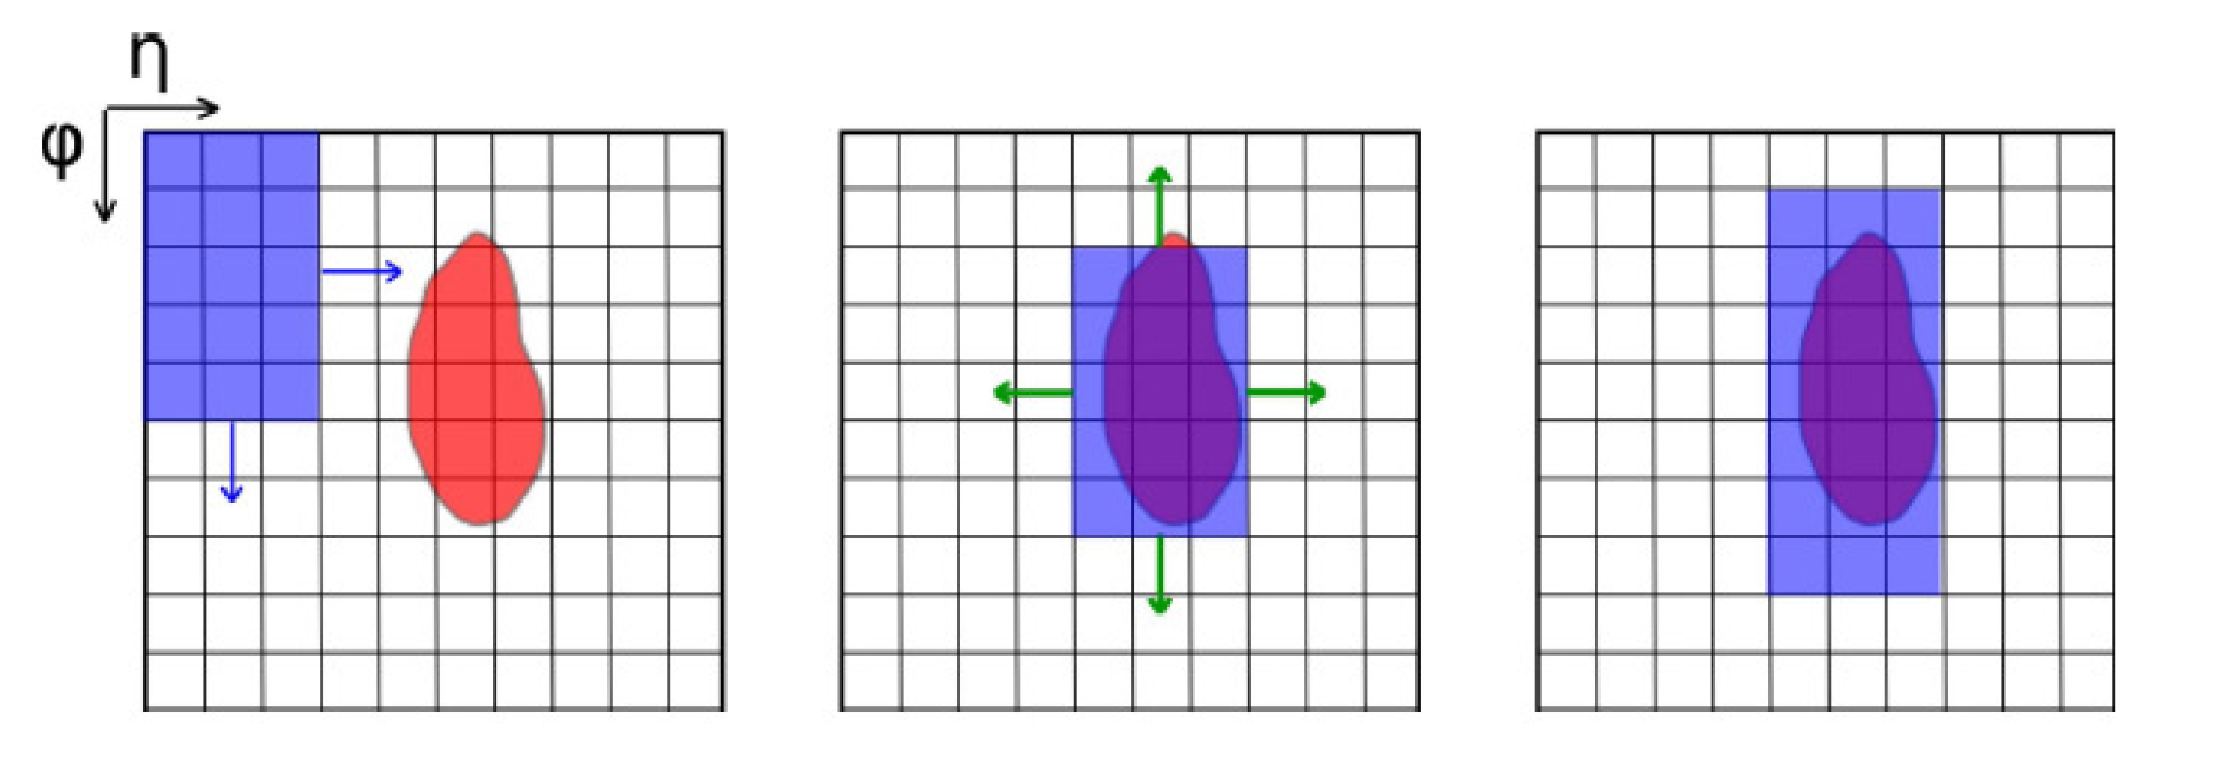
\includegraphics[width=0.85\textwidth]{objectsreconstruction/figures/slidingwindow}}
	\caption{The three steps of the sliding window algorithm.
	\label{fig:sliding}}
\end{center}\end{figure}

\section{Electrons}\label{sec:electrons}

Electrons~\cite{eperf} are reconstructed for pseudorapidities up to $|\eta| = 2.47$, where
information from the ID is available, matching a track (see Section~\ref{sec:tracks}) 
with a cluster in the electromagnetic calorimeter reconstructed with the sliding window 
algorithm (see Section~\ref{sec:clusters}).
In order to account for bremsstrahlung losses the matching is done within a region
of dimension $\Delta\eta\times\Delta\phi=0.05\times0.10$ and if more candidate
tracks are matched, of all the ones with hits in the silicon detectors
the track with the smallest $\dr$ with respect to the
energy cluster is chosen. In addition, the track momentum has to be compatible
with the cluster energy, which is calibrated to the electromagnetic scale
derived from Monte Carlo based corrections (to account for dead material losses),
test-beam studies and calibration from $Z\to ee$ events~\cite{Abat:1900zz}.

In general, electron can be distinguished from hadrons thanks to various characteristics
of their shower development: electrons deposit the most of their energy in the second layer of
the EM calorimeter; the width of their shower is narrower; they have smaller
hadronic leakage\footnote{The hadronic leakage is the ratio of the transverse energy reconstructed
in the first layer of the hadronic calorimeter to the total  transverse energy reconstructed in the 
EM calorimeter.}; the $E/p$ variable (ration of cluster energy and track momentum) is higher.

Some difficulties arise when dealing with $\pi^0$ and $\eta$ particles, which decay into two $\gamma$s
that produce two close showers reconstructed as a single one in the second layer of the EM
calorimeter, and in general with jets faking electrons from, e.g. QCD processes.
There are then six different electron definitions to help separate real electrons from fake ones,
described in the following ordered from the looser requirements to the tightest.
Performance studies on electron reconstruction and identification where done using 2010 data and Monte
Carlo $Z\to ee$ and $W\to e\nu$ events~\cite{eperf} (see Figure~\ref{fig:eleeff}). 

\texttt{Loose} electrons lie in the pseudorapidity region $|\eta| < 2.47$ and have 
low hadronic leakage and requirements on the variables defining the shower shape.
The identification efficiency is high but the jet rejection is low (about 500).

\texttt{Loose++} electrons are \texttt{loose} electrons whose track has at least one hit in 
the pixel detector and at least 7 hits in the combined silicon detectors and the
$|\eta_{\rm first EM}|$ distance between the track estrapolated to the first EM layer and
the matched cluster is lower than 0.015. The identification
efficiency is similar to the loose one but the rejection is ten times higher.

\texttt{Medium} electrons are \texttt{loose++} electrons where additional requirements on shower shape
are made as well as on their tracks: $|d_0|<$5~mm and $|\eta_{\rm first EM}|<0.01$.
The efficiency drops to 88\% and the rejection is
higher than the previous.

\texttt{Medium++} electrons are \texttt{medium} electrons whose track has at least one hit in the
first pixel detector layer, a requirement that allows to reject electrons from
photon conversion. Charged hadrons contamination is reduced by discarding candidates
whose track has a low fraction of high-threshold TRT hits. In addition, $|\eta_{\rm first EM}|<0.005$ 
and stricter cuts are applied to shower shaper of clusters in $|\eta|<2.01$. The
efficiency is about 85\% and rejection is about 50$\times 10^3$.

\texttt{Tight} electrons are \texttt{medium++} electrons with additional requirements on the distance
between the track and the matched cluster ($|\Delta\phi|<0.02$, $|\Delta\eta|<0.005$) and on the $E/p$
variable. Stricter cuts are imposed on the fraction of high-threshold TRT hits and on the impact parameter
($|d_0|<$1~mm). The efficiency drops to 75\% and the rejection is higher than the previous one.

\texttt{Tight++} electrons are \texttt{tight} electrons with asymmetric $\Delta\phi$ cuts, which give
both better efficiency and rejection.

\begin{figure}[tb]\begin{center}
	\subfigure[]{\label{fig:eleeffET}
  	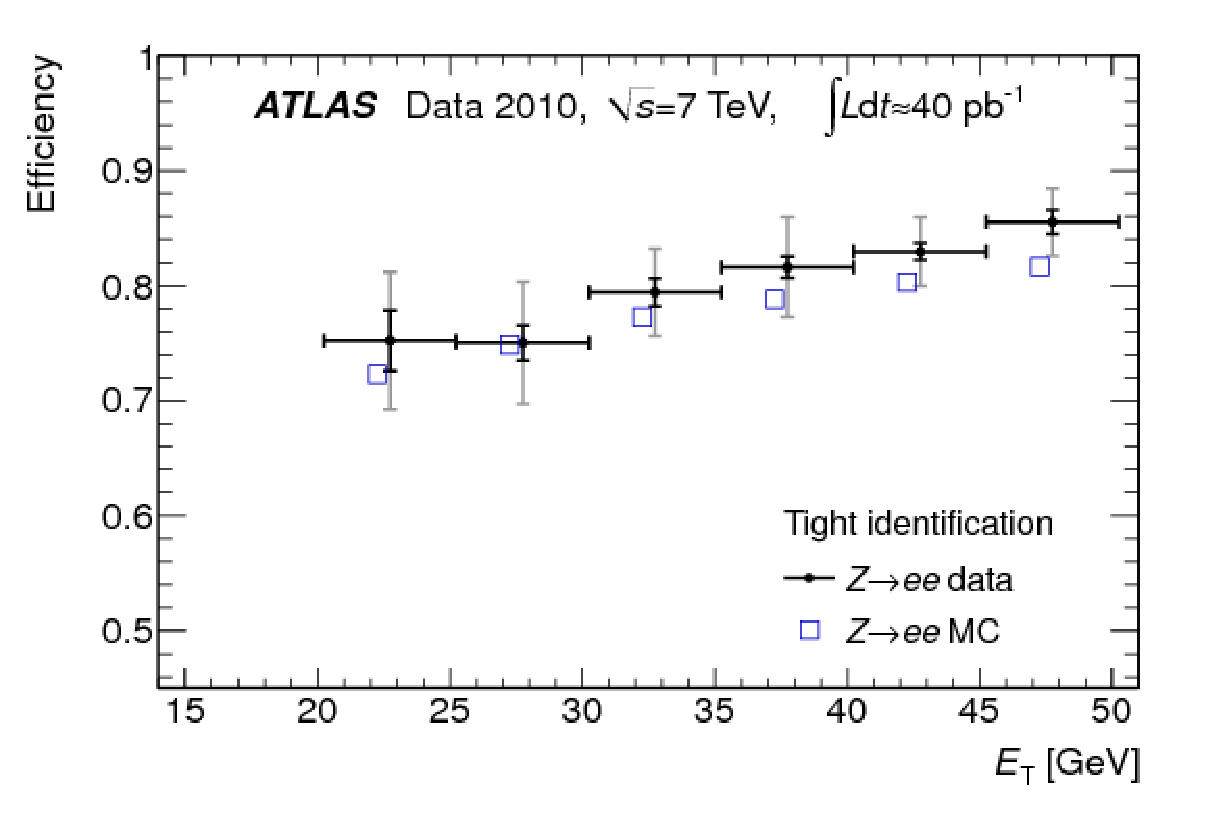
\includegraphics[width=0.45\textwidth]{objectsreconstruction/figures/Figures_EffZee_ET_tight_v2}}
	\subfigure[]{\label{fig:eleeffETA}
  	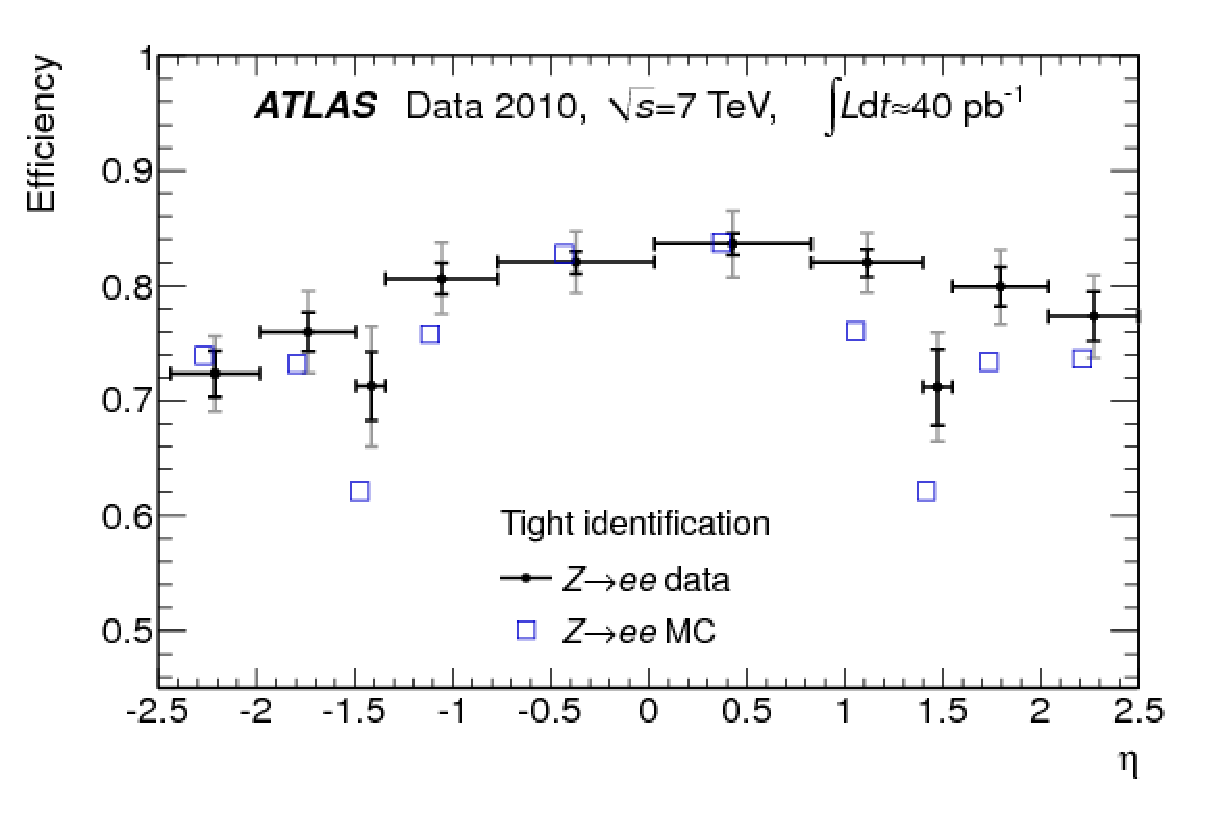
\includegraphics[width=0.45\textwidth]{objectsreconstruction/figures/Figures_EffZee_eta_tight_20to50_v2}}
	\caption{\texttt{Tight} electron identification efficiencies measured from $Z\to ee$ events and predicted by MC as a function (left) of~\ET\ (integrated over $|\eta|< 2.47$ excluding the transition region $1.37< |\eta|<1.52$ and (right) of~$\eta$ and integrated over $20< \ET<50$~GeV.~\cite{eperf}\label{fig:eleeff}}
\end{center}\end{figure}


\tocless\subsection{Additional requirement and corrections for analyses}\label{sec:REQtrigger}

For our analyses~\cite{topcommon2013}, electrons in the transition region $1.37<|\eta_{\rm cluster}| <1.52$
with inactive material are excluded. Electrons are required to satisfy \texttt{tight++} criteria and to
 have $\et = E_{\rm cluster}/\cosh\eta_{\rm track} > 25\gev$ and $z_0<2~$mm.
In addition, to suppress further the QCD multijet background, 
isolation cuts are imposed both as calorimeter (using the energy in a cone of size $\Delta R<0.2$, \texttt{EtCone20})
and track isolation (using the scalar sum of $p_T$s from tracks within a cone of $\Delta R<0.3$, \texttt{PtCone30}).
%isolation cuts to reduce the background from non-prompt electrons coming from
%hadron decays are defined, one based on the energy from calorimeter cells surrounding the candidate in
%a cone of radius $R=0.2$ and the other based on the track transverse momenta sum in a cone of radius $R=0.3$ around
%the electron.
The \texttt{EtCone20} and \texttt{PtCone30} isolation cuts are chosen to give
90\% efficiency.
In addition, jets (see Section~\ref{sec:jets}) within $\dr =0.2$ of the selected electron are 
discarded, and if an additional jet with $p_T>25~$\gev\  and $|JVF|>0.5$ is found within $\dr =0.4$,
then the electron is rejected.
The electron is matched to the single electron trigger \texttt{EF\_e24vhi\_medium1}
combined with a logical \texttt{OR} to the \texttt{EF\_e60\_medium1} trigger, which
recovers some efficiency loss at $\ET > 80$~GeV.

The efficiency in selecting electrons can be factorized as:
\begin{equation}\label{eq:eleeff}
\varepsilon = \varepsilon_{\rm reco} \cdot\varepsilon_{\rm tight++} \cdot\varepsilon_{\rm isolation} \cdot\varepsilon_{\rm trigger} 
	\end{equation}
where the various components represent respectively: the efficiency in recostructing the electron 
in terms of track-cluster match, track quality and hadronic leakage; the efficiency
for the \texttt{tight++} identification criteria; the efficiency for the isolation cuts;
the efficiency from trigger selection. Scale factors are derived in bins of $(\eta, \ET)$,
and the trigger scale factors are separated into four data-taking periods 
(\texttt{A-B3}, \texttt{B4-D3} without \texttt{C1-C5}, \texttt{C1-C5} and \texttt{D4+}).
The efficiency scale factors are applied as weights to Monte Carlo events.

The electron energies in data are corrected using scale factors $\alpha(\eta)$ derived
from data-to-simulation comparison in $Z\to ee$ events in order to match the $Z$ boson 
mass peak.

\section{Muons}\label{sec:muons}

As suggested in Figure~\ref{fig:decaychart}, muons interact with all of ATLAS sub-detectors,
even though they act as minimum ionizing particles (mip) for the calorimeters and hence will deposit
only a very small fraction of their energy in the material. Their track instead is precisely
measured both in the ID and in the muon spectrometer (MS). Based on how we decide to combine
the various information, we can list the following types of reconstructed muons:
\texttt{standalone} muons take the MS track and extrapolate it back to the interaction point;
\texttt{combined} muons match the MS track with the tracks from the ID;
\texttt{segment tagged} muons extrapolate ID tracks to the spectrometer and match the result with MS segments;
\texttt{calorimeter tagged} muons extrapolate ID tracks to the calorimeters and match the result with
energy deposits. 

We will only consider \texttt{combined} muons, recontructed using an algorithm called \texttt{Muid}~\cite{ATLAS-CONF-2011-063}
and whose pseudorapidity is limited to $|\eta|<2.5$ by the ID acceptance.
Starting from $\Delta\eta\times\Delta\phi=0.4\times0.4$ regions where interesting activity has been triggered,
track segments are searched for in the RPC and TGC and combined into a single track by means of a
least-square fitting method. These track candidates are hence extrapolated back to the interaction
point and their momentum corrected for the mip energy loss in the calorimeter material.

At this points a \chisq test (checking the difference between the extrapolated track coordinates weighted with
combined covariance matrix) on the matching of the candidate MS track and the tracks reconstructed in 
the ID is performed to obtain the final muon candidate track. Only ID tracks that satisfy some quality 
requirements are considered for the matching: they need to have at least two pixel hits, of which at least
one in the first layer; at least two pixel hits plus number of crossed dead pixel sensors; at least six SCT hits
plus number of  crossed dead SCT sensors; maximum two pixel or SCT holes\footnote{A ``hole'' in the silicon
detectors is a region where the module did not perform as expected even though the surrounding ones did.};
defining the number of TRT outliers\footnote{``Outlier'' is an hit that is deviated from the track path.} 
and the number of TRT hits as $N_{\rm TRT_{o}}$ and  $N_{\rm TRT_{h}}$ respectively, 
$N_{\rm TRT_{h}}>5$ and $N_{\rm TRT_{o}}/N_{\rm TRT_{h}}<0.9$ for $|\eta|<1.9$, 
$N_{\rm TRT_{o}}/N_{\rm TRT_{h}}<0.9$ if $N_{\rm TRT_{h}}>5$ for  $|\eta|\geq1.9$.
In case no matching is found, no
muons are reconstructed, while if more candidates arise, the one giving the best \chisq is chosen.
The momentum is computed as a weighted average of ID and MS measurements.

Performance studies on muon reconstruction and identification where done using 2010 data and Monte
Carlo $Z\to \mu\mu$ events~\cite{ATLAS-CONF-2011-063} (see Figure~\ref{fig:mueff}). 


\begin{figure}[tb]\begin{center}
	\subfigure[]{\label{fig:mueffET}
  	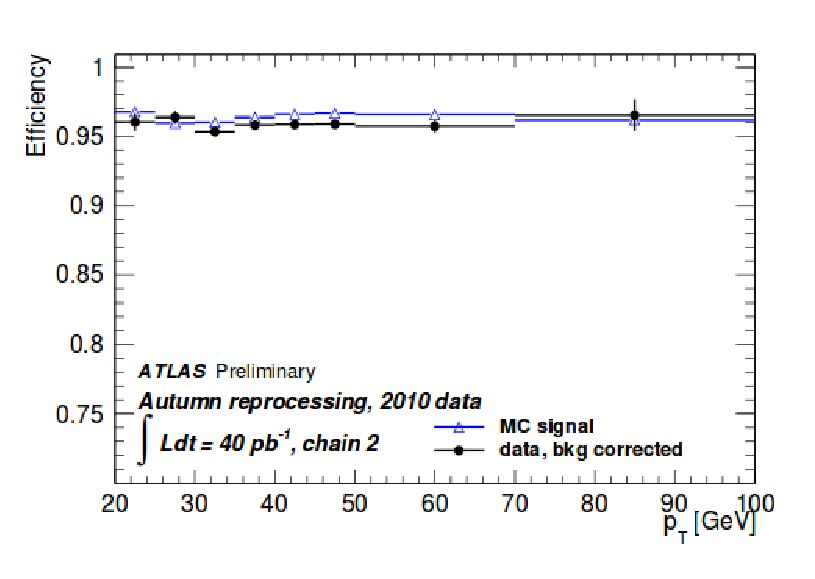
\includegraphics[width=0.45\textwidth]{objectsreconstruction/figures/Figures_EffZmumu_pt}}
	\subfigure[]{\label{fig:mueffETA}
  	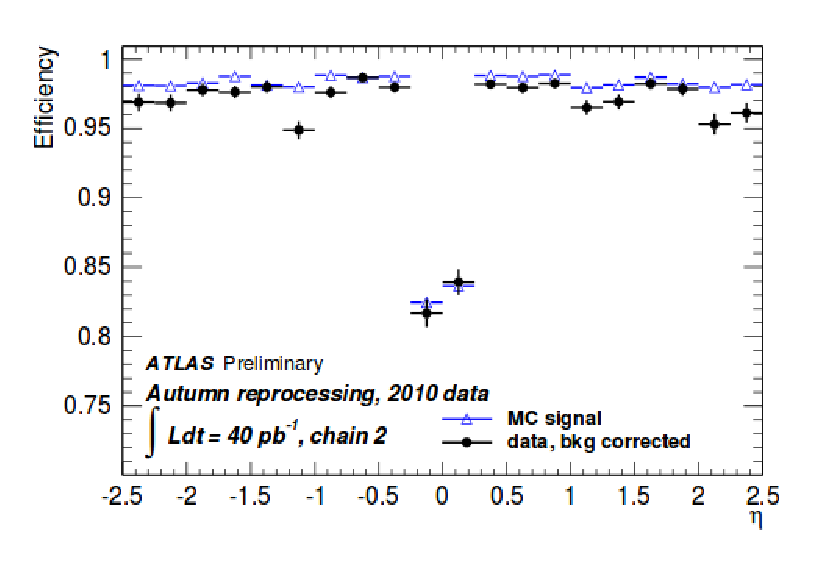
\includegraphics[width=0.45\textwidth]{objectsreconstruction/figures/Figures_EffZmumu_eta}}
	\caption{\texttt{Combined} muon reconstruction efficiencies using the \texttt{Muid} algorithm measured from $Z\to \mu\mu$ events and predicted by MC as a function (left) of~\pt\ and (right) of~$\eta$.~\cite{ATLAS-CONF-2011-063}\label{fig:mueff}}
\end{center}\end{figure}


\tocless\subsection{Additional requirement and corrections for analyses}

\texttt{Combined} muons are used in our analyses~\cite{topcommon2013} with an additional cut on the longitudinal impact
parameter $|z_0|<2~$mm to ensure the track comes  from the hard-scattering primary vertex.
A requirement on the muon momentum of $p_T>25$ is used to obtain 90\% efficiency from the chosen 
single muon trigger, which is the logical \texttt{OR} combination of the 
triggers \texttt{EF\_mu24i\_tight} and \texttt{EF\_mu36\_tight}. 
The \texttt{EF\_mu24i\_tight} trigger includes an isolation requirement 
for which the \pt\ sum of the tracks in a cone of size $\Delta R=0.2$  around the muon
has to be less than the 12\% of the muon transverse momentum.
Muons overlapping with any jet (see Section~\ref{sec:jets}) with $\pt>25$~GeV and $|JVF|>0.5$ 
within a $\Delta R<0.4$ cone are rejected.

In addition to the previous isolation requirements, a ``mini-isolation'' is 
defined~\cite{topcommon2013} to better deal with the high pile-up present
in $\sqrt{s} = $8~TeV collision events.
The mini-isolation is defined as 
\begin{equation}\label{eq:miniisol}
I_{mini}^{l} = \sum_{tracks} \pt^{track}/\pt^{l}
\end{equation}
where $\pt^{l}$ is the lepton transverse momentum and the summation runs over
all tracks found in a cone whose radius varies as a function of the muon momentum as:
\begin{equation}\label{eq:minicone}
\Delta R(l,track)=\dfrac{10\gev}{\pt^{l}}.
\end{equation}
The tracks also have to satisfy: $\pt^{track}>1~$GeV; $d_0 < 10$~mm;
$z_0 \sin\theta_{track} <10$~mm; at least four hits or dead sensors crossed in the silicon detectors.
The cut on the mini-isolation variable is chosen as $I_{mini}^{l}<0.05$
The performance of the mini-isolation is 
shown in Figure~\ref{fig:miniisoleff}.

\begin{figure}[tb]\begin{center}
	\subfigure[]{\label{fig:miniisolpt}
  	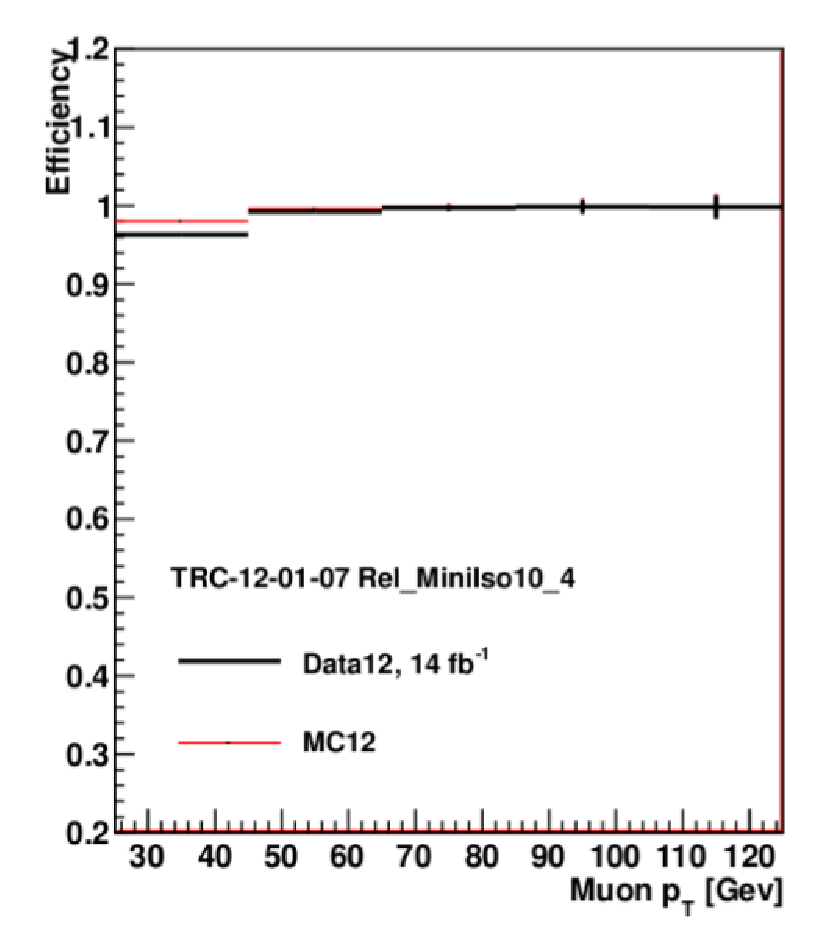
\includegraphics[width=0.45\textwidth]{objectsreconstruction/figures/miniisol_pt}}
	\subfigure[]{\label{fig:miniisolmu}
  	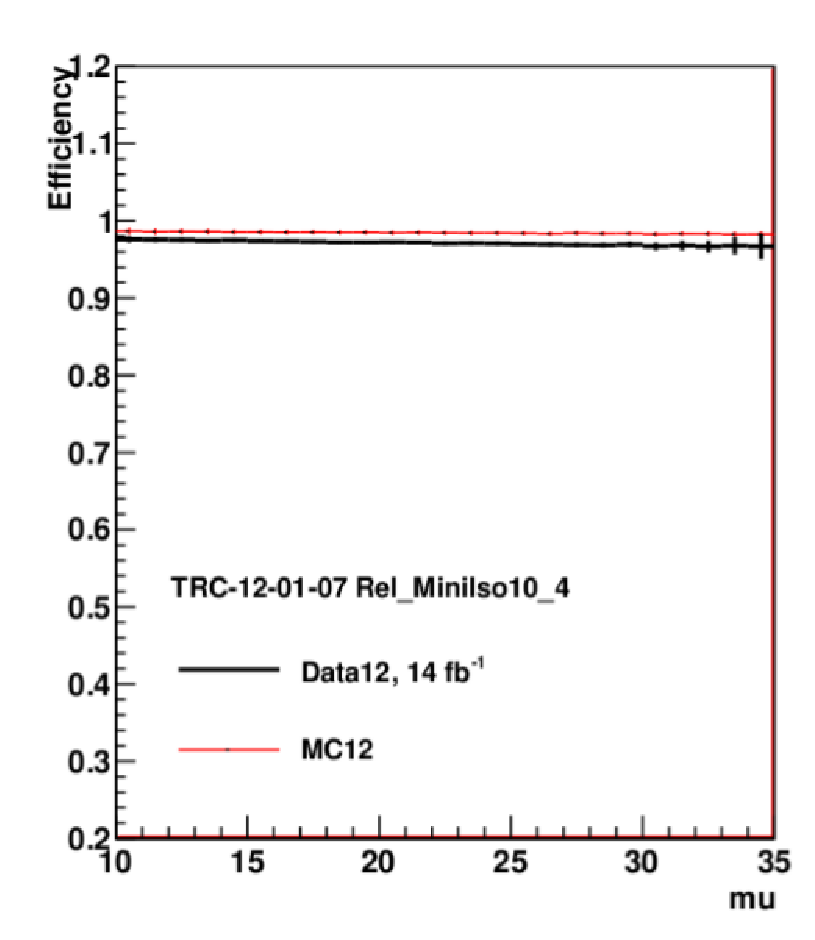
\includegraphics[width=0.45\textwidth]{objectsreconstruction/figures/miniisol_mu}}
	\caption{Efficiency of the mini-isolation as a function of the muon momentum (left) and of the average number
        of bunch crossings $<\mu>$ (right)~\cite{topcommon2013}.\label{fig:miniisoleff}}
\end{center}\end{figure}


As is done for electrons, a set of corrections are applied to correct for minor
discrepancies between Monte Carlo simulation and data events.
The scale factors to compensate recontruction, isolation and trigger i
nefficiencies are derived from tag-and-probe measurements
and applied to Monte Carlo events. In addition, the muon momentum
in simulated events is smeared to obtain agreement between the momentum
resolutions in Monte Carlo and data.


\section{Jets}\label{sec:jets}

With the name ``jet'' we generically refer to the object formed as a consequence
of parton hadronization from a spray (or {\it jet}) of particles. These particles
will leave signals both as tracks in the ID and as energy deposits in the calorimeters
and two type of jets can then be defined using either the former or the latter information:
track jets and calorimeter jets. In the following, we will only deal with calorimeter jets.

In order to interpret the detector information, first topoclusters are formed from the
calorimeter cells signals, as explained in Section~\ref{sec:clusters}. Then, different
algorithms were developed to associate topoclusters into a jet. Because of the
need for a stable and precise performance over the QCD processes from p-p collisions,
a set of requirements has been defined for the algorithms to be valid~\cite{Salam:2009jx}.

First of all, the splitting of one particle into two collinear particles must not change the 
result of the algorithm reconstruction, as well as the presence of additional soft emission.
The importance of Infrared and Collinear (IRC) safety is evident considering e.g. 
that a hard parton, as part of the fragmentation process, will undergo many collinear splittings,
and that QCD events always include emission of some soft particles, perturbatively or not.
In addition, we want the algorithm result to be invariant under Lorentz boost along the beam direction,
to be as insensitive as possible to detector effects like noise or resolution, and to be light in terms
of computing resourse usage.

A set of jet algorithm that satisfy these requirements are the sequential recombination
algorithms~\cite{ref:Cacciari2008,ref:Cacciari2006,ref:fastjet}, which combine topoclusters
into jets using as criteria a distance parameter defined as:
\begin{equation}
d_{ij}=min(p_{T_i}^{2p},p_{T_j}^{2p})\frac{\Delta R_{ij}^{2}}{R^{2}},
\end{equation}
\begin{equation}
d_{i}=p_{T_i}^{2p},
\end{equation}
where $p_{Ti}$ is the transverse momentum of topocluster $i$, 
$\Delta R_{ij}$=$\sqrt{\Delta\eta^{2}+\Delta\phi^{2}}$ the distance 
between constituents $i$ and
$j$, $R$ a parameter of the algorithm that approximately controls the size
of the jet, $p$ the parameter that defines the type of algorithm as:
\begin{equation}\label{eq:jetalgp}
\begin{array}{lcl}
p = 1 &:& k_t {\rm\ algorithm};\\
p = 0 &:& {\rm Cambridge/Aachen algorithm};\\
p = -1 &:& {\rm anti-}k_t {\rm\ algorithm}.
\end{array}
\end{equation}

The algorithms compute $d_{ij}$, the distance between the two topocluster
inputs $i$ and $j$, and $d_{i}$,  the distance between the input $i$
and the beam axis in the momentum space.
By computing the minimum of the two distances the choice made is
to combine $i$ and $j$ into a new input if $d_{ij}<d_{i}$, or take
$i$ as a jet candidate and remove it from the input list if $d_{i}<d_{ij}$. 
The cluster combination is done by summing the four-momentum of each input.
The distances are recalculated with the updated list of input
objects and the process repeated until no further cluster is left.

The anti-$k_t$ algorithm is chosen by most of analyses in ATLAS as it is particularly 
performant against pile-up, since it starts summing up 
constituents with higher momentum, and produces jets with a conical
structure (see Figure~\ref{fig:jetshapes}).

\begin{figure}[tb]\begin{center}
	\subfigure[]{\label{fig:jetshapes}
  	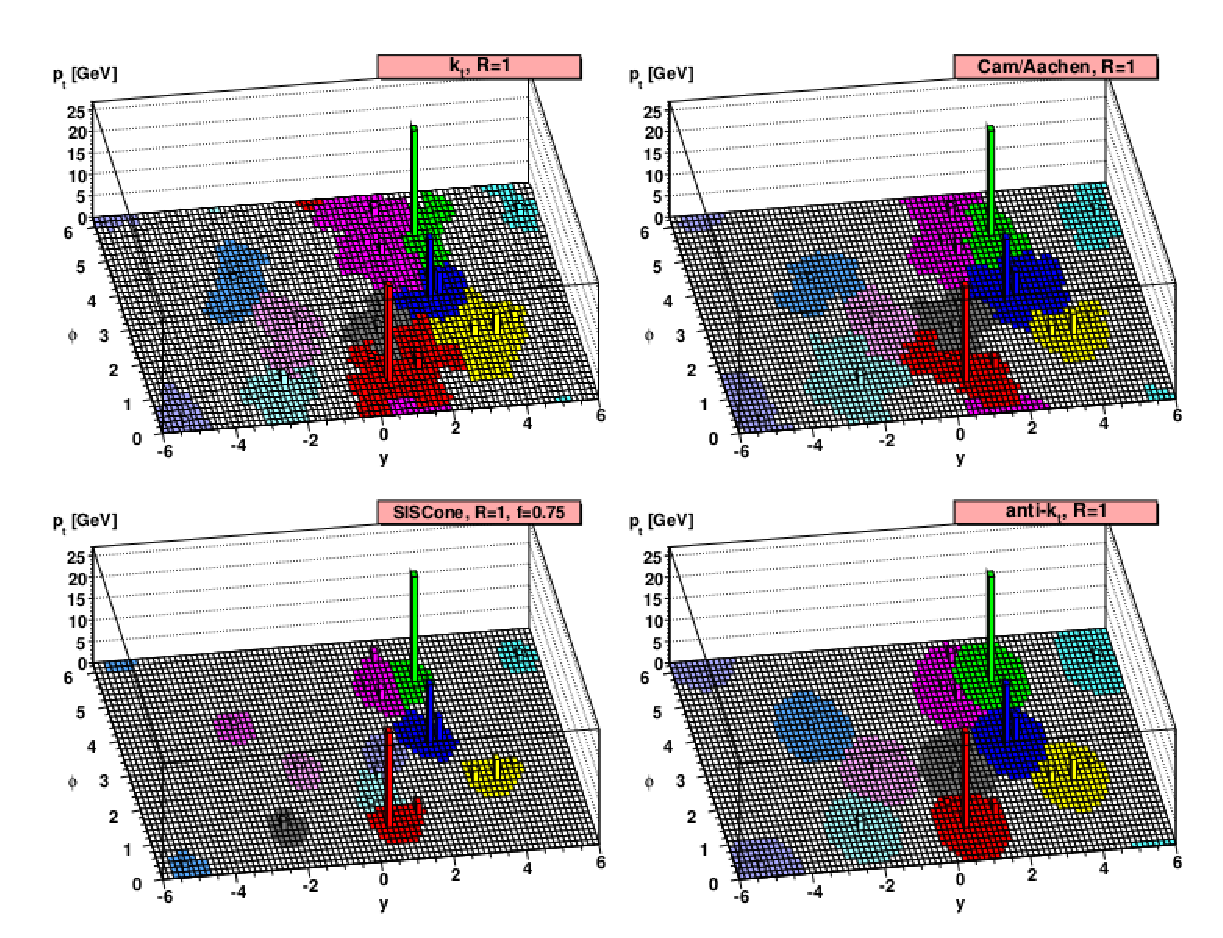
\includegraphics[width=0.5\textwidth]{objectsreconstruction/figures/jetshapes}}
        \subfigure[]{\label{fig:corr_jet}
        \includegraphics[width=0.47\textwidth]{objectsreconstruction/figures/corr_jet_lcw.eps}}
        \caption{Left: The same input produces different results in terms of jet reconstruction using 
        various jet algorithms~\cite{Salam:2009jx}. Right: Average jet energy response from simualted events
        at the LCW scale for various calibrated energies ($E$) as a function of
        pseudo-rapidity. The inverse of the response shown 
        in each bin is equal to the average jet energy scale correction~\cite{jes}.}
\end{center}\end{figure}


\tocless\subsection{Additional requirement and corrections for analyses}

For our analyses~\cite{topcommon2013} jets are reconstructed using the anti-$k_t$
algorithm with a radius parameter $R=0.4$ (from which the algorithm is often referred to as anti-$k_t$4) 
using calorimeter energy deposits corrected for effects of non-compensation\footnote{The energy response 
to hadrons is lower than the response to electrons of the same energy due to the presence of invisible processes.},
dead detector material and out-of-cluster leakage.
Other effects affecting jet energy are low momentum particles
that are deflected by the magnetic field and energy losses in 
topocluster formation and jet reconstruction~\cite{jes}. 

The initial energy is reconstructed at the electromagnetic (EM) scale as
the calorimeter signals arise from electromagnetic interaction of
particles with matter. The energy calibration to EM scale was derived
during test-beam runs using electron beams, validated with muons
from both test-beam and cosmic-rays runs and corrected using simulated $Z\to ee$ events.

Of the several energy calibration schemes derived in ATLAS, we will be using the 
Local Cluster Weighting (LCW) calibration~\cite{LCW1,LCW2}.
This scheme exploits properties of the topoclusters shapes 
to classify the clusters as ``mainly electromagnatic'' or
``mainly hadronic'' and then derives the calibration from Monte Carlo simulation
of charged and neutral pion events. The calibration corrections are applied
before the jet reconstruction algorithm is operated, and after the jet is
formed a final correction is applied to ensure linearity in response.

%hmmmmmm AAAAAAAAA anche a 8 tev???
%To subtract contributions from in-time and out-of-time pile-up interactions a correction is applied
%parameterized according to the number of primary vertices in the event and the number of average interactions 
%in the luminosity block ($<\mu>$) as a function of jet pseudorapidity.

In our analyses we consider only jets with $\pt > 25\gev$ and $|\eta| < 2.5$.
Furthermore, a variable called ``jet vertex fraction" (JVF) is defined as the fraction
of the sum of $\pt$ of tracks with $\pt>1\gev$
associated with the jet that comes from tracks originating from the primary vertex.
By requiring JVF$>0.5$ we avoid selecting jets from in-time pile-up events.

To avoid double counting of energy deposits from electrons as jets,
if jets are found within $\Delta R$ of 0.2 of the selected electron, the
jet closest to the lepton is removed and then electrons that lie within $\Delta R< 0.4$ of
the remaining jets are discarded.


\subsection{$b$-tagging}~\label{sec:btagging}

When a bottom quark is produced in an events, it hadronizes into a $B$ hadron, which has
a lifetime of the order of $10^{-12}$~s and hence can travel about 3~mm before decaying.
The result is a displaced secondary vertex that, if correctly reconstructed, can
allow for the identification of the bottom quark. 
Since this capacity relies on track reconstruction from the ID, its applicability
is limited by the ID acceptance to the pseudorapidity region $|eta|<2.5$.

\begin{figure}[tb]\begin{center}
	\subfigure{
  	\includegraphics[width=0.5\textwidth]{objectsreconstruction/figures/Picture-b-tagging-2}}
	\caption{Simple schematic of the displaced secondary vertex.\label{fig:btagvtx}}
\end{center}\end{figure}

This technique is called $b$-tagging~\cite{ref:ATLAS-CONF-2011-102} and is
widely used in ATLAS analyses with top quarks. There are three types of algorithms,
and they can be combined to obtain better performance. In general they define a weight
corresponding to the probability for the jet to be tagged, and a working point is chosen
as the threshold for this weight to discriminate between $b-$ and not-\bjet s
by finding a good compromize between a good efficiency (the ratio between tagged
$b$-jets and true $b$-jets) and a high light-jet rejection
(the inverse of the number of light-jets misidentified as $b$-jets).

Algorithms like \texttt{IP1D}, \texttt{IP2D} and \texttt{IP3D} are
based on information from impact parameters of the tracks
contained in the jet, $z_0/\sigma_{z_0}$, $d_0/\sigma_{d_0}$ and a
combination of the two respectively. A likelihood is computed to
obtain the $b-$tag weights.

Other algorithms reconstruct the secondary vertex from the $B$ hadron
decay, allowing for a better discrimination between \bjet s and light
jets. The \texttt{SV1} algorithm uses the number of track pairs in
the secondary vertex, their total invariant mass and the ratio of
the sum of the energies of tracks from the secondary vertex to the one
of the total tracks of the jet to compute likelihood ratios the logarithm
of which are then summed to obtain the $b-$tag weights.

Finally, the \texttt{JetFitter} algorithm uses the full decay chain reconstruction
of $b$ and $c$ hadrons by fitting it with a Kalman filter to determine a 
common path between the primary vertex and the vertices from the $b$ and $c$ hadrons 
inside the jet. The likelihood is computed with the flight length significances
of the vertices and the variables from the  \texttt{SV1} algorithm.

The algorithm emploied in our analyses is called \texttt{MV1} and uses
a neural network to combine information from the \texttt{JetFitter}, \texttt{IP3D}
and \texttt{SV1} algorithms.
The working point corresponding to 70\% efficiency, 
$\sim$130 light-jet rejection and a charm-jet rejection of 5 is 
chosen (see Figure~\ref{fig:btageffs}).

\begin{figure}[tb]\begin{center}
	\subfigure{
  	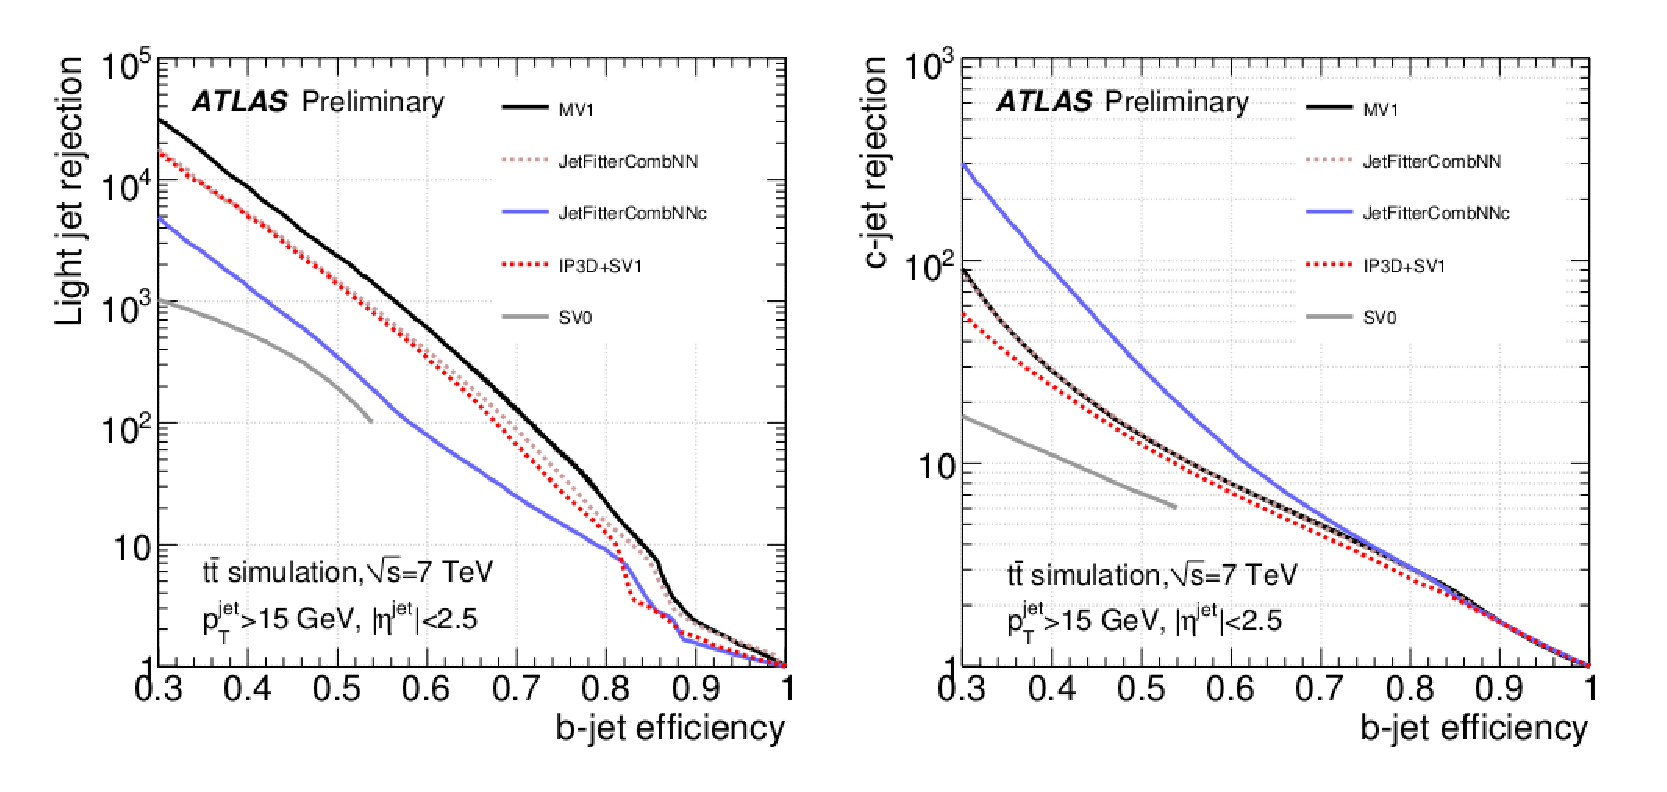
\includegraphics[width=0.8\textwidth]{objectsreconstruction/figures/btageffs}}
	\caption{Light- (left) and $c-$jet (right) rejection as a function of the \bjet\ tagging efficiency
        for different tagging algorithms. These values refer to jets with $\pt >15\gev$ and 
$|\eta|<2.5$ in simulated $t\bar{t}$ events~\cite{btagging}.\label{fig:btageffs}}
\end{center}\end{figure}

The tagging efficiencies in Monte Carlo are corrected for $b$ and $c$ flavours
with the appropriate $\epsilon_{data}/\epsilon_{MC}$ scale factors,
determined in bins of jet $\pt$ and $\eta$.

\subsubsection{Tag Rate Function method}\label{sec:trf}

When requiring $\geq 1$ $b$-tagged jet the
available Monte Carlo statistics is significantly reduced for 
some particular background processes, leading to large
fluctuations in the resulting distributions.
% This can negatively
%affect the sensitivity of the analysis, as the corresponding
%statistical uncertainties on the background templates need to be taken
%into account in the determination of exclusion limits, and lead to
%unreliable systematic uncertainties in the predicted distribution
%shapes. In addition, the observed limits may be biased, depending on
%how the MC distributions fluctuate with respect to the data in the
%signal region.


To overcome this problem the Tag Rate Function (TRF) method is introduced.
Here, no event is rejected based on its $b$-tagging count, but instead all the events are 
kept and weighted according to the
probability of the given event to contain the desired number of \bjet s.
The event weight is computed based on the kinematics and flavour of the jets found in each event
and using the tagging efficiency, which is a function of $\eta$, $\pt$ and true jet flavour.

Given a jet with $\eta$, $\pt$ and flavour $f$, its tagging probability can be noted as:
\begin{equation*}
        \varepsilon \left(f,|\eta|,\pt\right)
\end{equation*}

For a given event with $N$ jets, its probability of containing exactly one $b$-tag jet can be computed as:
\begin{equation*}
        P_{=1} = \sum\limits_{i=1}^N \left( \varepsilon_{i} \prod\limits_{i \neq j} \left( 1 - \varepsilon_{j} \right) \right)
\end{equation*}

In the same way, it can be used to compute the probability for inclusive $b$-tag selections:
\begin{align*}
        P_{=0} &= \prod\limits_{i=1}^N \left( 1 - \varepsilon_{j} \right) \\
        P_{\geq 1} &= 1 - P_{=0}
\end{align*}

Since this method relies on the correctness of the tagging efficiency,  closure tests have been performed to check
calibration of the tagging efficiency in Monte Carlo samples. These studies show that the efficiency parametrization
officially provided~\cite{topcommon2013}  is not as accurate as expected, and therefore new efficiency maps where
obtained. With correct calibrations the average of the histogram of $1/\varepsilon$ vs $\eta$, $\pt$ and true jet flavour 
should be flat and with mean equal to one. Figure~\ref{fig:closure} shows these variables using the official and the new maps.
%As it can be observed, there are departures from closure of to up to 40\% in some regions of the light flavor map, and on average 13\%.
%New efficiency maps have been derived using a combination of $t\bar{t}$ {\sc MC@NLO}, $t\bar{t}$ {\sc Alpgen}, and {\sc Protos} $\TT$ MC samples.
%Figure~\ref{fig:closure} shows reasonably good closure for the newly derived efficiency map.
%The new efficiency map will therefore be used for the probability computations in the TRF method.
It is clear that some regions of the light flavor map show high departure from closure, hence the
new efficiency map will be used for the probability computations in the TRF method.

\begin{figure}
  \begin{center}
  \begin{tabular}{c c}
    \includegraphics[width=0.45\textwidth]{objectsreconstruction/figures/TRFmethod/5closureRebin.eps} &
    \includegraphics[width=0.45\textwidth]{objectsreconstruction/figures/TRFmethod/5myclosureRebin.eps} \\
    \includegraphics[width=0.45\textwidth]{objectsreconstruction/figures/TRFmethod/4closureRebin.eps} &
    \includegraphics[width=0.45\textwidth]{objectsreconstruction/figures/TRFmethod/4myclosureRebin.eps} \\
    \includegraphics[width=0.45\textwidth]{objectsreconstruction/figures/TRFmethod/0closureRebin.eps} &
    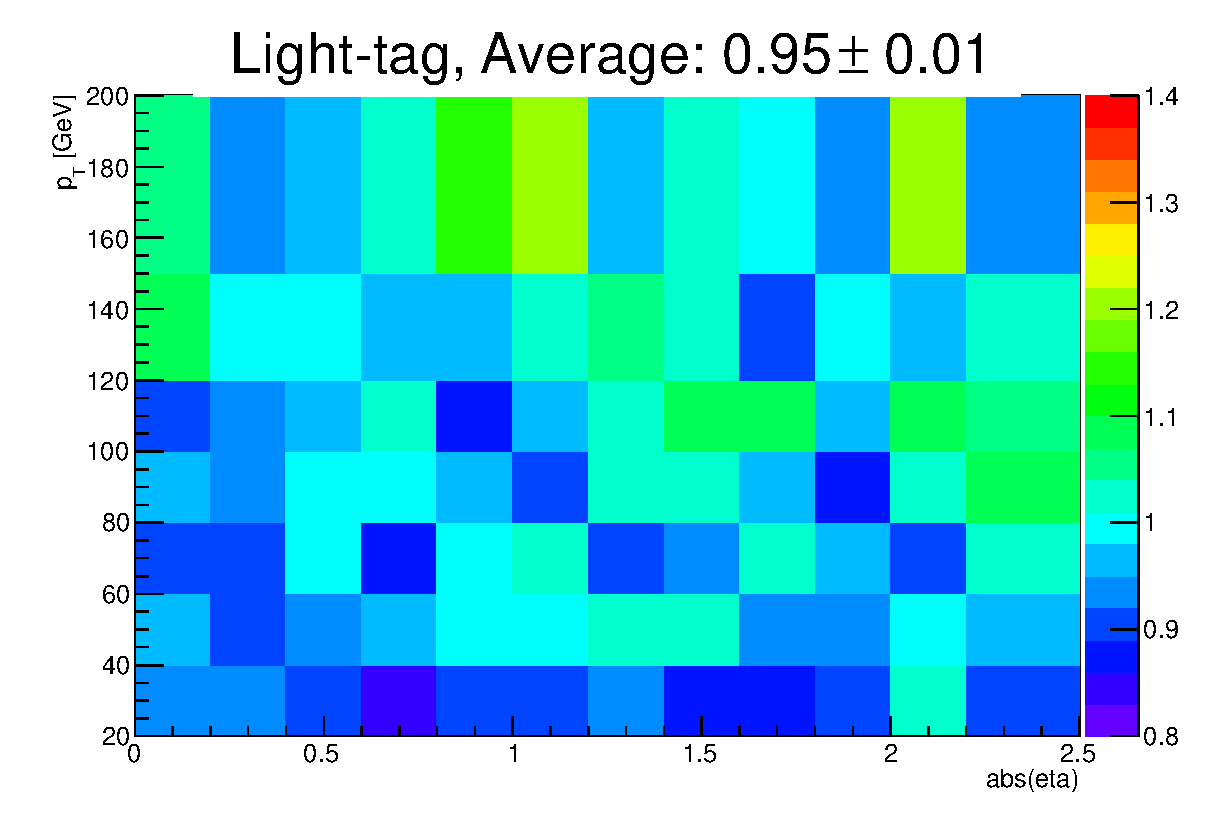
\includegraphics[width=0.45\textwidth]{objectsreconstruction/figures/TRFmethod/0myclosureRebin.eps} \\
  \end{tabular}
  \end{center}
  \caption{Results of the closure test using efficiency from the official calibration file 
  (left column) and the private efficiency map (right column). The test is split in the
 different jet flavours: $b$ jets (top), $c$ jets (middle) and light jets (bottom). }
  \label{fig:closure}
\end{figure}




\section{Missing Transverse Energy}\label{sec:met}

To estimate the momentum of invisible particles in the event, i.e. neutrinos and, eventually, new particles,
the missing transverse energy $\met$~\cite{met} is defined~\cite{topcommon2013} to balance the total transverse momentum of the event.
Indeed, while the longitudinal energy of the interacting partons is unknown, as they carry an unpredictable
fraction of the total proton momentum, its transverse component is, initially, zero.
Possible sources of fake contributions to the \met\ are detector coverage, dead or noisy regions and
finite detector resolution.

The \met\ is computed by first matching each calorimeter energy 
deposit is with a high-$\pt$ object,  in the following order: electrons, photons, jets and muons.
These are respectively the RefEle, RefGamma, RefJet, RefMuon terms, wether the low-$\pt$ jets
are grouped into the SoftJet term. Then, the energies of these objects are
corrected accordingly to the respective calibration constants. 
The calorimeter clusters
that did not get associated with any  high-$\pt$ object are calibrated for energy losses in 
dead material regions and for the different response to the electromagnetic and hadronic
components of particle showers and added as the CellOut term. 
Finally the \met\ is computed as:
\begin{equation}\label{eq:met}
\begin{array}{lcl}
E^{\rm miss}_{x,y} & = & E^{\rm RefEle}_{x,y} + E^{\rm RefGamma}_{x,y} + E^{\rm RefJet}_{x,y} + E^{\rm RefMuon}_{x,y} + E^{\rm SoftJet}_{x,y} + E^{\rm CellOut}_{x,y}\\
E^{\rm miss}_{T} & = & \sqrt{(E^{\rm miss}_{x})^2 + (E^{\rm miss}_{y})^2}\\
\end{array}	\end{equation}

%\subsection{Additional requirements for analyses}
